\documentclass{article}
\usepackage{graphicx}
\usepackage[margin=1.5cm]{geometry}
\usepackage{amsmath}

\begin{document}

\title{Warm Up: Unit 1 Kinematics}
\author{Prof. Jordan C. Hanson}
\maketitle

\section{Memory Bank}
The following formulas apply to systems experience \textit{constant acceleration}, $a$.  That is, $a = 0$, or $a = $ constant, but it does not depend on time.
\begin{enumerate}
\item If $a = 0$, then $v = \frac{x_f - x_i}{t_f - t_i}$, and $v$ is constant.
\item If $a \neq 0$, then $v(t) = a t + v_i$ ... This is the velocity of a system at a time $t$, with acceleration ($a$) times time, plus initial velocity $v_i$.
\item If $a \neq 0$, $x(t) = \frac{1}{2}a t^2 + v_i t + x_i$ ... This is the position of a system at time $t$, equal to one-half the acceleration ($a$) times time ($t$) squared, plus initial velocity ($v_i$) times time, plus initial position ($x_i$).
\end{enumerate}

\section{Chapters 2.3 - 2.5}

\begin{enumerate}
\item Graphically, the velocity is the slope of position versus time.  In Fig. \ref{fig:1}, a system moves initially in the positive x-direction, but is experiencing constant negative acceleration.  Eventually, it is moving in the negative x-direction.  (a) What is the velocity (the slope) at $t_0$? (b) Is the average velocity between $t_1$ and $t_6$ greater than, less than, or equal to the instantaneous velocity at $t_0$? (c) Suppose $t_1$ and $t_6$ are equal to 0.5 and 3.5 seconds, respectively.  If $x_1$ and $x_6$ are the corresponding positions, equal to 1 and 5 meters, respectively, what is the average velocity, $v$ between $t_1$ and $t_6$?
\begin{figure}[hb]
\centering
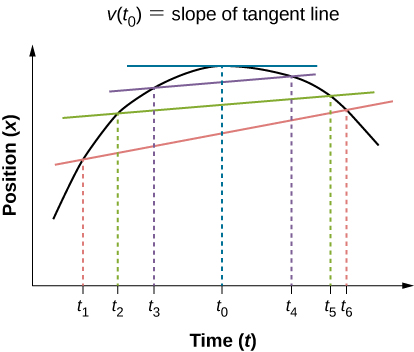
\includegraphics[width=0.33\textwidth]{figures/slope.jpeg}
\caption{\label{fig:1} A system moves initially in the positive x-direction, experiencing negative acceleration.}
\end{figure}
\item From the memory bank, we see that the formula that accurately descibes the position of accelerating systems versus time is a quadratic formula.  Using what you know about $t_1$, $t_6$, $x_1$, and $x_6$, determine the quadratic equations that correctly describes Fig. \ref{fig:1}.  (\textit{Assume $x(0) = 0$} and that $a$ is negative).
\end{enumerate}

\end{document}
